\begin{figure}
    \centering

    \subfigure[主动语态]{\label{fig5-1-1}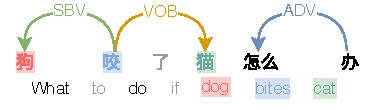
\includegraphics[scale=1.1]{figure/fig5-1-1.pdf}}

    \subfigure[被动语态(复述关系)]{\label{fig5-1-2}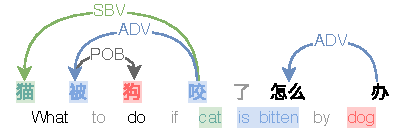
\includegraphics[scale=1.1]{figure/fig5-1-2.pdf}}

    \subfigure[被动语态(非复述关系)]{\label{fig5-1-3}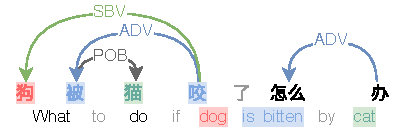
\includegraphics[scale=1.1]{figure/fig5-1-3.pdf}}
    \caption{主被动语态依存关系图}
    %Same words are with same color between example and corresponding translation.
    %'SBV'' to Subject-Predicate relation, 'ADV' refers to the relationship between adverbial and head word and 'POB' referfs to the relationship between preposition and object.
    \label{fig5-1}
\end{figure}